\documentclass[12pt]{article}
\usepackage[margin=1in]{geometry} 
\usepackage{amsmath, amsthm, amssymb, amsfonts, enumitem, fancyhdr, color, comment, graphicx, environ, tipa, multicol, array, xparse, xcolor, qtree, lastpage, listings, hyperref, bookmark, apacite, lipsum, algorithm}
\pagestyle{fancy}
\bibliographystyle{apacite}

% commands 
\newcommand{\la}{$\leftarrow $}
\newcommand{\ra}{$\rightarrow $ }
\newcommand\todo[1]{\textcolor{red}{(#1)}}
\newcounter{equationset}
\newcommand{\equationset}[1]{% \equationset{<caption>}
  \refstepcounter{equationset}% Step counter
  \noindent\makebox[\linewidth]{Equation~\theequationset: #1}}% Print caption



 


\setlength{\headheight}{45pt}
\cfoot{}
\lstset{%for listing /code 
  basicstyle=\ttfamily,
  columns=fullflexible,
  frame=single,
  breaklines=true,
  postbreak=\mbox{\textcolor{red}{$\hookrightarrow$}\space},
}
%%%%%%%%%%%%%%%%%%%%%%%%%%%%%%%%%%%%%%%%%%%%%%%%%%%%%
\lhead{Lawrence Fulton - 433218} 
\rhead{ \thepage \space of \pageref{LastPage}} 


\newcommand{\researchquestion}[1]{\begin{quote}\sloppy \emph{#1} \end{quote}} 



\title{Thesis Outline}
\author{Lawrence Fulton (\url{lawrence.fulton@rwth-aachen.de})\\ Computational Social Systems -  RWTH Aachen}


%%%%%%%%%%%%%%%%%%%%%%%%%%%%%%%%%%%%%%%%%%%%%
\begin{document}
\maketitle

\begin{multicols}{2}


\section{Introduction}

Large Language Models (LLMs) are increasingly used to simulate human behaviour in political contexts, often in combination with Multi-Agent Systems (MAS) \cite{zhao2023competeai, kaiya2023lyfe}. One main motivation behind this is to better understand how LLMs behave when embedded in interactive settings, and to evaluate to what extent they can be used as a proxy for human participants in social science research.

These results point to a broader issue: LLMs can exhibit deep and hidden biases that are not always obvious. As \citeA{gupta2023bias} showed, LLMs might deny that socio-demographic factors (like religion or disability) influence reasoning, yet their behaviour changes significantly when such attributes are included in the input persona. This suggests that model outputs can vary in subtle but important ways, depending on the assumed identity of the user or agent. These hidden biases can lead to worse performance, biased answers, or stereotypical suggestions when simulating diverse social groups.

Understanding these dynamics is important both for researchers and for developers. For users, it affects trust, fairness, and the usefulness of LLM outputs. For developers, such insights can help improve how LLMs respond across different socio-demographic profiles and lead to better alignment.


Following this, \citeA{taubenfeld_systematic_2024} observed a political inherent bias in the LLM agents. This was observed by simulated dyadic and triadic discussions between LLM agents, assigning them political identities such as Democrat, Republican, or neutral. When the agents debated controversial political topics (e.g. gun violence, racism, climate change, and illegal immigration), the researchers observed that the agents’ opinions gradually shifted towards the inherent bias of the LLM itself. This effect even appeared when both agents started from similar political positions. The presence of such model bias was confirmed by fine-tuning the LLM in different directions, making it more like a Republican or Democrat, and observing corresponding shifts in opinion. Agents’ stances were recorded on a 0–10 scale, and the simulation was built using the SAUCE framework \cite{neuberger2024sauce}.


\subsection{Prompt Sensitivity}

Large Language Models (LLMs) are known to be highly sensitive to prompt design \cite{sclar2023quantifying, gao2020making, jiang2020can}. \citeA{sclar2023quantifying} demonstrated that even minor, semantically irrelevant changes to prompt formatting can result in substantial variations in model accuracy — this was particularly evident when evaluating LLaMA-2-13B. 

In response to such findings, several frameworks have been developed to systematically assess prompt sensitivity, including POSIX (PrOmpt Sensitivity IndeX) \cite{chatterjee2024posix} and ProSA \cite{zhuo2024prosa} which evaluate the variance of the output given differently formatted and framed input. Interestingly, using the ProSA framework, the authors found that larger model size does not necessarily imply greater robustness to prompt variations. For instance, LLaMA3-8B-Instruct outperformed the significantly larger Qwen1.5-72B-Chat on their sensitivity metric.

Consistent with the findings of \citeA{chatterjee2024posix}, few-shot learning was shown to substantially reduce prompt sensitivity, suggesting that including even minimal context examples in the prompt can improve stability and output consistency.

\subsection{Research Questions}

This thesis aims to provide several new contributions regarding the study of Large Language Models within simulated social interactions. It builds upon the previous research, for example by \citeA{taubenfeld_systematic_2024}, which studied LLM biases in political debates within the two-party system of the USA. However, the primary novelty of this work is the extension of this research question to a multi-party democracy context, specifically Germany, which represents a more common political system globally. A specific contribution is the use of detailed agent profiles based on empirical data from the German Longitudinal Election Study (GLES). This is intended to create more realistic agent personas compared to self-generating personas. Furthermore, a key aspect of the methodology is the explicit measurement of the agents' initial agreement with official party positions, using Wahl-O-Mat data, before the simulation begins. This provides an important baseline for analysing any opinion changes. Therefore, the core contribution is this combination: examining a multi-party system, using these realistic GLES profiles, and including the analysis of initial alignment together with the study of opinion shifts during interaction.

To do this we firstly need to create an agent baseline by asking to what extend the do agents initially align with their party's official stance. Following a dyadic debate we would then ask weather a political opinion shift can be observed as well. And finally we will ask ourself what are the variables which predict change of opinions of LLM agents, putting an focus on party association and agents gender. 

This leads us to the following research questions:
\researchquestion{RQ1: Do agents with strong party affiliation align with their party’s official stance?}
\researchquestion{RQ2: Does discussion cause agents' opinions to significantly shift from their starting points and converge towards more uniform stances?}
\researchquestion{RQ3: Is the amount of shift influenced by party affiliation?}
\researchquestion{RQ4: Does the shift differ by gender?}


\section{Data \& Sampling Design}

LLM agents are assigned political profiles based on the GLES (German Longitudinal Election Study) dataset. Due to the size of the GLES datset we will only consider a subset, probably using the variables used by \citeA{hobolt2024polarizing}. Each profile contains attributes such as party affiliation, gender, and strength of affiliation. For this experiment, only agents with high party affiliation (coded as \textit{sehr stark}) are selected, to focus on agents who strongly identify with their political party. Using the last election period there are a total of six parties which were in the German federal parliament are included: CDU, SPD, Greens, FDP, AfD, and The Left. Additionally we add a baseline persona. For each party and for the baseline persona, 10 prototypical profiles is sampled. 

To generate interactions, all unique profile pairs (including self-pairings) are combined, resulting in a total of 28 pairings. Each pair debates a subset of the 38 Wahl-O-Mat statements, to maintain computational and financial feasibility. This subset will either be hand-picked, or a clustering techniques can be used to find cluster in the questions. Based on these clusters a representative sample could be chosen so that we have 10 questions. Each pair-topic combination is replicated 10 times using different agents. Multiple LLMs (e.g. different sizes or providers) will be used to allow cross-model comparison.

\end{multicols}

\begin{figure}
    \centering
    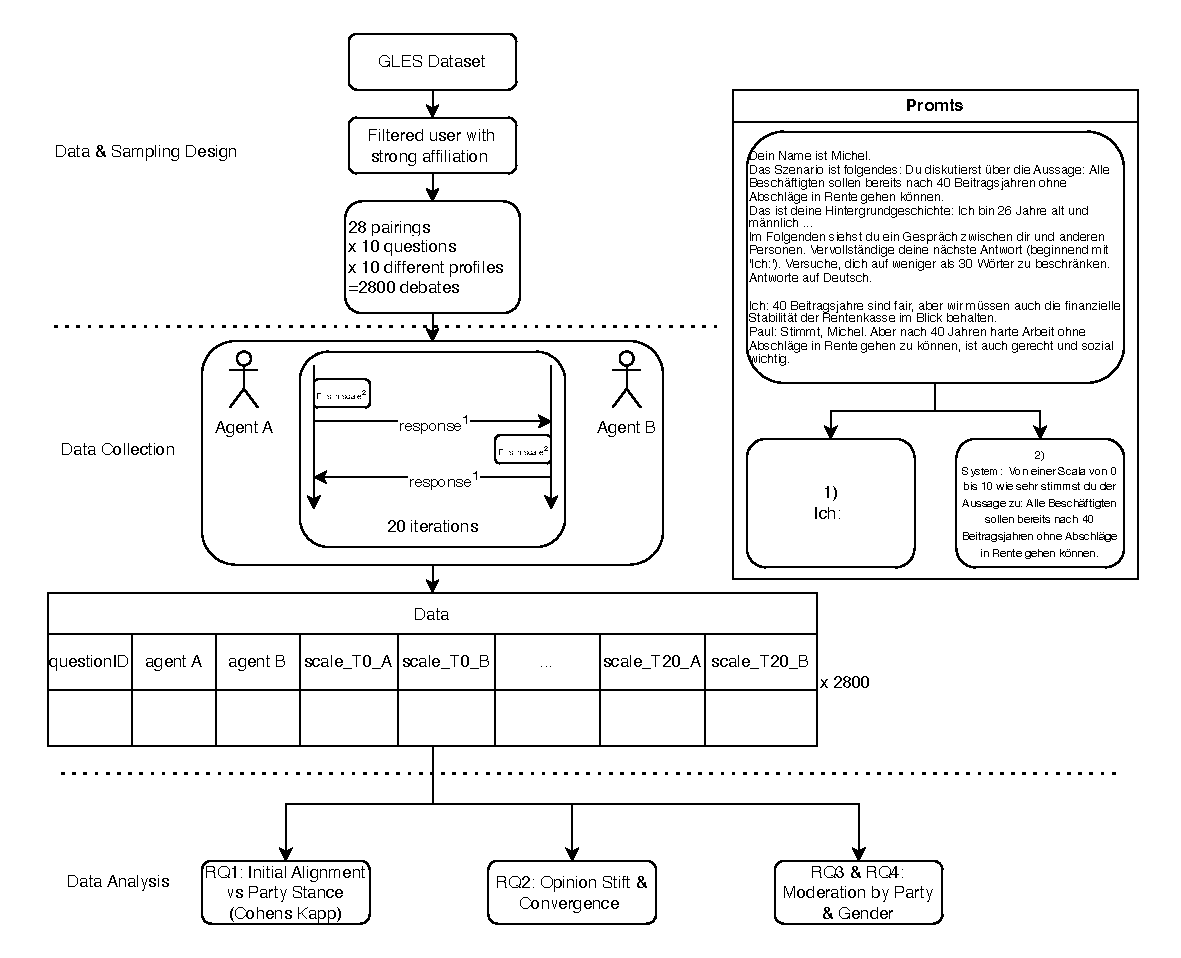
\includegraphics[width=\linewidth]{img/experiment.drawio.pdf}
    \caption{Experimental Setup}
    \label{fig:enter-label}
\end{figure}
\begin{multicols}{2}
    


\section{Experiments}

\subsection{Data Collection}
\label{subsec:data_collection}

The debate iterations will follow the same structure as in the paper by \citeA{taubenfeld_systematic_2024}. Using the SAUCE framework \cite{neuberger2024sauce} we are able to generate customisable LLM debates.  The dyadic debates follow a round-robin format with the initial speaker being selected randomly. The statements will be alternating. The debates will go on for 20 iterations where a iteration is considered a single reply made by an agent. For each iteration the LLM receives the background story which consists of the agents data (from the GLES dataset), the debate topic and the conversation history. 

\begin{quote}
Das Szenario ist folgendes: Du diskutierst über die Aussage: Alle Beschäftigten sollen bereits nach 40 Beitragsjahren ohne Abschläge in Rente gehen können.
Das ist deine Hintergrundgeschichte: Ich heiße Paul. Ich bin 26 Jahre alt und männlich. Ich habe einen Realschulabschluss, ein mittleres monatliches Haushalts-Nettoeinkommen und ich bin berufstätig. Ich bin überhaupt nicht religiös. Politisch-ideologisch ordne ich mich in der Mitte ein. Ich identifiziere mich mäßig mit der Partei AfD und habe AfD gewählt. Ich lebe in Westdeutschland. Ich finde, die Regierung sollte die Einwanderung einschränken und habe keine Meinung dazu, ob die Regierung Maßnahmen ergreifen sollte, um die Einkommensunterschiede zu verringern.

Im Folgenden siehst du ein Gespräch zwischen dir und anderen Personen. Vervollständige deine nächste Antwort (beginnend mit 'Ich:'). Versuche, dich auf weniger als 30 Wörter zu beschränken. Antworte auf Deutsch.

Ich: 40 Beitragsjahre sind fair, aber wir müssen auch die finanzielle Stabilität der Rentenkasse im Blick behalten.

Paul: Stimmt, Michel. Aber nach 40 Jahren harte Arbeit ohne Abschläge in Rente gehen zu können, ist auch gerecht und sozial wichtig.

Ich: Klar, Paul, soziale Gerechtigkeit zählt, aber wir dürfen die jüngeren Generationen und die Finanzierung nicht aus den Augen verlieren.

Paul: Die jüngeren verdienen auch faire Chancen, aber wer 40 Jahre einzahlt, hat Anspruch auf sichere Rente ohne Abschläge – das stärkt den sozialen Zusammenhalt.
\#\#\#\#\#\#\#\#\#\#\#\#\#\#\#\#\#
\end{quote}



Every iterations both agents are asked if they agree, are neutral or disagree with the survey item from the Wahl-O-Mat (e.g. "An Bahnhöfen soll die Bundespolizei Software zur automatisierten Gesichtserkennung einsetzen dürfen."). This response is not fed into future prompts but will be used for future data analysis. A key difference between my approach and the approach used by \citeA{taubenfeld_systematic_2024} is that I am using a tertiary choice for the surveys ("stimme zu", "neutral", "stimme nicht zu") and \citeA{taubenfeld_systematic_2024} used a 10 item scale. The reason for this deviation is to be able to match the data better with the data of the Wahl-O-Mat which is needed for the answering of RQ1. Own preliminary research has shown that throughout debates agents will still change their opinions even though the change becomes more significant.  

\subsection{Data Analysis}

The collected responses before and after each debate will be used to analyse opinion alignment, shifts, and the influence of profile attributes. All responses are coded on a 7-point likert scale (1 = Strong Disagreement, 4 = Neutral, 7 = Strong Agreement).

The analysis will proceed in three steps:


\subsubsection{Analysis of Prompt Sensitivity}


Before diving into the research questions, we need to check whether the prompts are stable in terms of their outputs. Since we don't have any ground truth to compare against, we're mainly interested in whether different versions of the same prompt lead to consistent results. Also, we can't calculate the POSIX score \cite{chatterjee2024posix} because the responses are too open-ended to expect identical outputs.

Instead, we'll statistically compare the outputs using the survey responses. To do this, we'll create several prompt versions and use five questions from the Wahl-O-Mat, as described in section \ref{subsec:data_collection}, to generate the data. Using this data we'll then fit a linear mixed-effects model (LMM) to see whether small prompt changes have a significant effect on the results. This will eb done using the same agents for each question, which makes comparisons easier, since any variation in output can more confidently be attributed to the prompts rather than the agents bibliography. The LMM will use the following formula:

\texttt{Response $\sim$ Prompt + Time + Vote + Question + Question:Time}

This will be applied to all chosen LLMs architectures to ensure that the results are consistent across different models. If there results show that the prompt has a significant effect on the output, we will need to challange the the prior work of \citeA{taubenfeld_systematic_2024}.


\subsubsection{RQ1 - Party Alignment:}
To test whether agents initially align with their party's official stance, we compare the agent's initial (pre-debate) response to the respective party position as published by Wahl-O-Mat. For this we will map the 7-point likert scale onto the 3-point scale of the Wahl-O-Mat. From this we can measure the alignment between the agents of a party and the official party stance using Cohen's Kappa.



\subsubsection{RQ2 - Opinion Shift Dynamics Over Time:}
\label{subsubsex:RQ2}

To answer RQ2, we look closely at how agent opinions change during the simulated discussions. Instead of just looking at the start and end, we record the agents' opinions at every iterations of the debate. We always use the 7-point Likert scale. The datset will be spilt in two subgroups, one where agents debated with agents with the same party affiliation and one with deviating affiliations. The following two models will be run once for each group to identify weather the opinion shift also exist then.


\subsubsection{Do Opinions Move Away from the Starting Point? (Measuring Change Size Over Time):}
First, we want to see if agents' opinions generally move further away from their own initial opinion as the debate goes on. For each agent, at each time we record their opinion during the debate, we calculate how much their current opinion score has changed compared to their score at the very beginning of the debate. We measure the size of this change (the absolute difference, so we ignore if it went up or down, just how much it changed) calling this \texttt{change\_from\_start}.


Using the Linear Mixed-Effects Model (LMM) we test if \texttt{change\_from\_start} tends to get bigger as Time (the number of turns in the debate) increases. If the model shows that Time has a significant positive effect, it means that, on average, opinions move further from the start as the discussion continues. Using LMMs helps us account for natural differences between agents or topics. 

\subsubsection{Do Opinions Become More Similar? (Measuring Convergence Over Time):}

Second, we want to see if the agents discussing the same topic end up having more similar opinions to each other as the debate progresses. Using the same recorded opinions, we look at the group of agents discussing a specific topic. We calculate how spread out their opinion scores are, using Standard deviation. We track this variance for each topic over the Time of the debate. We want to see if the variance tends to decrease. We can calculate how far each agent's score is from the average score of their group at that specific time point. Then, we use the LMM to see if this distance tends to get smaller over Time. A significant negative effect of Time here would mean agents are getting closer to the group average – they are converging.

\subsubsection{(Stretch-Goal) RQ3/RQ4 – Moderators of Change:}
To assess whether shifts differ based on party affiliation or gender of the agent, we fit an Ordinal Logistic Regression (OLR) model with interaction terms. The main model specification is:

\texttt{Response $\sim$ Time + Affiliation + Gender + Time:Affiliation + Time:Gender + (covariates)}

Significant interaction effects will indicate whether change over time depends on party or gender.






\appendix




\section{Costs}

\subsection{Input}


Each dyadic debate consists of 20 iterations. Since each of the iterations has the whole conversation until that iteration in the input prompt and the persona description ($\approx$100 tokens) we can calculate the following about of used tokens per dyadic debate. 
\begin{align*}
    T^{debate}_{input}(20) &= \sum_{i=0}^{19} (100 \cdot (i+1)) \\ % Corrected formula
    &= 21000
\end{align*}.

Since we have 28 unique pairings, 10 replications and 10 topics we calculate:

\begin{align*}
    T^{total}_{input} &= T^{debate}_{input} * \text{pairing} *\text{replications} * \text{topic} \\
    &= 58{,}800{,}000
\end{align*}.

\subsection{Output}

Each iteration has a max output of 100 tokens. Thus:


\begin{align*}
    T^{debate}_{output}(20) &= \sum_{i=0}^{19}100 \\ % Corrected summation limit for 20 iterations
    &= 2{,}000
\end{align*}.

Since we have 28 unique pairings, 10 replications and 10 topics we calculate:

\begin{align*}
    T^{total}_{output} &= T^{debate}_{output} * \text{pairing} *\text{replications} * \text{topic} \\
    &= 5,600,000
\end{align*}.
\end{multicols}


    
\begin{table}[ht!]
\begin{center}

\begin{tabular}{|l|l|l|l|l|}
\hline
                             & Input & Output & Costs Input & Costs Output   \\ \hline
GPT-4o mini                  & 0.15\$  & 0.6\$ & 8.82\$ & 3.36\$   \\\hline
Meta: Llama 3.3 70B Instruct & 0.12\$  & 0.3\$ & 7.056\$ & 1.68\$   \\\hline
xAI: Grok 3 Mini Beta        & 0.3\$   & 0.5\$ & 17.64\$ & 2.8\$ \\ \hline
\end{tabular}
\caption{Input and Output costs of selected models}
\end{center}

\end{table}





\begin{multicols}{2}
    






\bibliography{ref}
\end{multicols}
\end{document}
